\chapter{Kiến Thức Nền Tảng}
\ifpdf
    \graphicspath{{Chapter2/Chapter2Figs/PNG/}{Chapter2/Chapter2Figs/PDF/}{Chapter2/Chapter2Figs/}}
\else
    \graphicspath{{Chapter2/Chapter2Figs/EPS/}{Chapter2/Chapter2Figs/}}
\fi

\begin{quote}

\textit{Trong chương này, chúng tôi sẽ trình bày những kiến thức nền tảng trên ba chủ đề bao gồm mạng nơ-ron hồi quy, Long short-term memory và mô hình ngôn ngữ nơ-ron. Mạng nơ-ron hồi quy (RNN) là xương sống của dịch máy nơ-ron. Nó được sử dụng để làm cả bộ mã hóa lẫn bộ giải mã. Ứng với mỗi vai trò, RNN sẽ có một thiết kế riêng. Long short-term memory là phiên bản cải tiến của RNN để giải quyết vấn đề về phụ thuộc dài hạn. Long short-term memory cũng là phiên bản RNN được dùng để xây dựng nên bộ mã hóa - bộ giải trong khóa luận này. Sau đó, dựa trên những kiến thức về mạng nơ-ron hồi quy, chúng tôi nói về khái niệm \textit{mô hình ngôn ngữ hồi quy} với chức năng tạo ra từ trong bộ giải mã, là bước quan trọng trong dịch máy nơ-ron. Những thành phần này cung cấp kiến thức nền tảng để đi đến mô hình dịch máy nơ-ron theo kiến trúc bộ mã hóa - bộ giải mã mà chúng tôi sẽ trình bày trong chương 3}.

\end{quote}
\section{Mạng nơ-ron hồi quy (Recurrent neural network)}

Trong tự nhiên, dữ liệu không phải lúc nào cũng được sinh ra một cách ngẫu nhiên. Trong một số trường hợp, chúng được sinh ra theo một thứ tự. Xét trong dữ liệu văn bản, ví dụ ta cần điền vào chỗ trống cho câu sau \textit{"Paris là thủ đô của nước \_\_"}. Dễ biết được rằng chỉ có duy nhất một từ phù hợp cho chỗ trống này, đó là \textit{"Pháp"}. Điều này có nghĩa là mỗi từ trong một câu không được tạo ra ngẫu nhiên mà nó được tạo ra dựa trên một liên hệ với những từ đứng trước nó. Các loại dữ liệu khác như những khung hình trong một bộ phim hoặc các đoạn âm thanh trong một bản nhạc cũng có tính chất tương tự. Những loại dữ liệu mang thứ tự này được gọi chung là dữ liệu chuỗi (sequential data).

Trong quá khứ, một số mô hình xử lý dữ liệu chuỗi bằng cách giả định rằng đầu vào hiện tại có liên hệ với một số lượng xác định đầu vào trước đó, nhiều mô hình tạo ra một cửa sổ trượt để nối mỗi đầu vào hiện tại với một số lượng đầu vào trước đó nhằm tạo ra sự mô phỏng về tính phụ thuộc. Cách tiếp cận này đã được sử dụng cho mô hình \textit{Deep belief network} trong xử lý tiếng nói \cite{massetal2012}. Nhược điểm của những cách làm này là ta phải xác định trước kích thước của cửa sổ. Một mô hình với kích thước cửa sổ với chiều dài bằng 6 không thể nào quyết định được từ tiếp theo trong câu \textit{"Hổ là loài động vật ăn \_\_"} sẽ là \textit{"thịt"} hay \textit{"cỏ"}. Trong ví dụ này, từ tiếp theo của câu phụ thuộc mật thiết vào từ \textit{"Hổ"} cách nó đúng 6 từ. Trên thực tế, có rất nhiều câu đòi hỏi sự phụ thuộc với nhiều từ xa hơn trước đó. Ta gọi những sự phụ thuộc kiểu như vậy là những \textit{phụ thuộc dài hạn} (long term dependency). 

\textit{Mạng nơ-ron hồi quy} (recurrent neural network) \cite{elman1990} gọi tắt là \textit{RNN} là một nhánh của nạng nơ-ron nhân tạo được thiết kế đặc biệt cho việc mô hình hóa dữ liệu chuỗi. Khác với những mô hình đã đề cập giả định sự phụ thuộc chỉ xảy ra trong một vùng có chiều dài cố định. RNN, trên lý thuyết, có khả năng nắm bắt được các phụ thuộc dài hạn với chiều dài bất kỳ. Để làm được điều đó, trong quá trình học, RNN lưu giữ những thông tin cần thiết cho các phụ thuộc dài hạn bằng một véc-tơ được gọi là \textit{trạng thái ẩn}.

Xét một chuỗi đầu vào $x={x_1,x_2,...,x_n}$. Ta gọi $h_t$ là trạng thái ẩn tại \textit{bước thời gian} (timestep) $t$, là lúc một mẫu dữ liệu $x_t$ được đưa vào RNN để xử lý. Trạng thái ẩn $h_t$ sẽ được tính toán dựa trên mẫu dữ liệu hiện tại $x_t$ và trạng thái ẩn trước đó $h_{t-1}$. Có thể thể hiện $h_t$ như một hàm hồi quy với tham số là đầu vào hiện tại và chính nó ở thời điểm trước đó:
\begin{equation} \label{basicRnnEquation}
	h_t = f \left(h_{t-1}, x_t \right)
\end{equation}
trong đó hàm $f$ là một ánh xạ phi tuyến. Có thể hình dung $h_t$ như một đại diện cho những đầu vào mà nó đã xử lý từ thời điểm ban đầu cho đến thời điểm $t$. Nói một cách khác, RNN sử dụng trạng thái ẩn như một dạng bộ nhớ để lưu giữ thông tin từ một chuỗi. Hình \ref{fig_rnn_loop} thể hiện định nghĩa hồi quy của RNN.

\begin{figure}
	\centering
	\includegraphics[width=0.25\textwidth]{rnn_loop}
	\caption[Mô hình RNN với kết nối vòng]{Mô hình RNN đơn giản với kết nối vòng, \textbf{$h$} được xem như bộ nhớ được luân chuyển trong RNN. Chú ý rằng đường nét đứt ở đầu ra thể hiện rằng tại một thời điểm $t$, RNN có thể có hoặc không có một đầu ra.}
	\label{fig_rnn_loop}
\end{figure}
Thông thường, hàm $f$ là một hàm phi tuyến như hàm \textbf{sigmoid} hay hàm \textbf{tanh}. Xét một RNN với công thức cụ thể như sau:
\begin{equation} \label{rnnWithTanh}
	h_t = \phi \left(W_{xh} x_t + W_{hh}h_{t-1} + b_h \right)
\end{equation}
Trong đó:
\begin{itemize}
	\item[•] $\phi$ là một hàm kích hoạt (ví dụ: sigmoid, tanh hay ReLU).
	\item[•] $h_{t} \in \mathbb{R}^n$ là trạng thái ẩn tại bước thời gian hiện tại.
	\item[•] $x_t \in \mathbb{R}^m$ là đầu vào hiện tại.
	\item[•] $h_{t-1} \in \mathbb{R}^n$ là trạng thái ẩn tại bước thời gian trước đó.
	\item[•] $W_{xh} \in \mathbb{R}^{m \times n}, W_{hh} \in \mathbb{R}^{n \times n}$ và $b_h \in \mathbb{R}^n$ lần lượt là hai ma trận trọng số và véc-tơ "bias".
\end{itemize}

Ma trận $W_{xh}$ là làm nhiệm vụ kết nối giữa đầu vào và trạng thái ẩn, $W_{hh}$ kết nối trạng thái ẩn với chính nó trong các bước thời gian liền kề. Véc-tơ $b_h$ dùng để điều chỉnh giá trị của $h_t$. Tại thời điểm bắt đầu, trạng thái ẩn $h_0$ có thể được khởi tạo bằng 0 hoặc là một véc-tơ chứa tri thức có sẵn như trường hợp của bộ giải mã như chúng tôi đã đề cập trong chương 1.

Tại mỗi bước thời gian $t$, tùy vào mục tiêu cụ thể của quá trình học mà RNN có thể có thêm một đầu ra $y_t$. Trong ngữ cảnh bài toán dịch máy nơ-ron, đầu ra của RNN trong quá trình giải mã chính là một từ trong ngôn ngữ đích hay nói chung là một đầu ra dạng rời rạc. Với mục tiêu đó, đầu ra dự đoán của RNN $\hat{y}_t$ sẽ có dạng là một phần phối xác suất trên tập các các lớp ở đầu ra. Phân phối này nhằm dự đoán vị trí xuất hiện của $\hat{y}_t$.
%\begin{equation} \label{rnnOuputSoftmax}
%	s_t = W_{hy}h_t + b_y
%\end{equation} 
\begin{equation} \label{rnnOuputSoftmaxDistribution}
	\hat{y}_t = \softmax(W_{hy}h_t + b_y)
\end{equation}
Trong đó:
\begin{itemize}
	\item[•] $\softmax$ là một hàm kích hoạt với $\softmax(v_j) = \frac{e^{v_j}}{\sum_{k=1}^{K}e^{v_k}}$, $j = 1,...,K$, $K$ là độ dài của véc-tơ $v$.
	\item[•] $h_{t} \in \mathbb{R}^n$ là trạng thái ẩn tại bước thời gian hiện tại.
	\item[•] $W_{hy} \in \mathbb{R}^{L \times n}$ và $b_y \in \mathbb{R}^L$ lần lượt là hai ma trận trọng số và véc-tơ "bias". $L$ là số lượng lớp cần phân biệt ở đầu ra.
\end{itemize}

Trong công thức trên, hàm $\softmax$ đóng vai trò là một hàm chuẩn hóa để $\hat{y}_t$ thể hiện một phân phối xác suất trên các lớp ở đầu ra. Ma trận $W_{hy}$ kết nối đầu ra với trạng thái ẩn, $b_y$ dùng để điều chỉnh giá trị của kết quả tính toán trước khi đưa qua hàm $\softmax$.

\begin{figure}
	\centering
	\includegraphics[width=0.85\textwidth]{rnn_unrolled}
	\caption[Mô hình RNN dạng dàn trải]{Mô hình RNN được dàn trải (unrolled), ví dụ trong 4 bước thời gian.}
	\label{fig_rnn_unrolled}
\end{figure}

Để ý rằng các ma trận trọng số $W_{xh}$, $W_{hh}$, $W_{hy}$ và các véc-tơ bias $b_h$, $b_y$ là các tham số học của mô hình và chúng là duy nhất. Có nghĩa là khi những tham số này được học, bất kỳ một đầu vào nào cũng đều sử dụng chung một bộ tham số. Điều này chính là sự chia sẻ tham số (parameters sharing) trong mạng nơ-ron hồi quy. Chia sẻ tham số khiến cho mô hình học dễ dàng hơn, nó giúp cho RNN có thể xử lý chuỗi đầu vào với độ dài bất kỳ mà không làm tăng độ phức tạp của mô hình. Quan trọng hơn, nó giúp ích cho việc tổng quát hóa. Đây chính là điểm đặc biệt của RNN so với mạng nơ-ron truyền thẳng.

Với một số lượng hữu hạn các bước thời gian, mô hình RNN trên hình \ref{fig_rnn_loop} có thể được dàn trải ra (unrolled). Dạng dàn trải này được miêu tả trực quan như trên hình \ref{fig_rnn_unrolled}. Với cách thể hiện này, RNN có thể được hiểu như là một mạng nơ-ron sâu với mỗi bước thời gian là một mạng nơ-ron một tầng ẩn và các tham số học được chia sẻ giữa các mạng nơ-ron đó. Dạng dàn trải cũng thể hiện rằng RNN có thể được huấn luyện qua nhiều bước thời gian bằng thuật toán lan truyền ngược (backpropagation). Thuật toán này được gọi là "Backpropagation through time" (BPTT) \cite{werbos1990}. Thực chất đây là chỉ thuật toán “Backpropagation” khi áp dụng cho RNN dưới dạng dàn trải để tính "gradient" cho các tham số ở từng bước thời gian. Hầu hết cả các mạng nơ-ron hồi quy phổ biến ngày nay đều áp dụng thuật toán này vì tính đơn giản và hiệu quả của nó.

\subsection{Huấn luyện mạng nơ-ron hồi quy}

Xét một chuỗi đầu vào $x={x_1,x_2,...,x_n}$ với đầu ra tương ứng $y={y_1,y_2,...,y_n}$. Trong quá trình lan truyền tiến, tại mỗi bước thời gian $t$ ứng mẫu dữ liệu $(x_t, y_t)$, công thức tính toán đầu ra dự đoán có dạng:
\begin{equation} \label{rnnForwardProp1}
	h_t = \phi \left(W_{xh} x_t + W_{hh}h_{t-1} + b_h \right) 
\end{equation}
\begin{equation} \label{rnnForwardProp2}
	s_t = W_{hy} h_t + b_y 
\end{equation}
\begin{equation} \label{rnnForwardProp3}
	\hat{y}_t = softmax (s_t) 
\end{equation}
Ta cần định nghĩa hàm độ lỗi giữa đầu ra dự đoán $\hat{y}_t$ và đầu ra thật sự $y_t$. Với $L$ là số lượng lớp của $y$, lúc này có thể thấy $\hat{y}_t$ là một véc-tơ phân phối xác suất có độ dài $L$. Để so sánh với $\hat{y}_t$, $y_t$ được chuẩn hóa thành một véc-tơ dạng "one hot" có nghĩa là một véc-tơ với độ dài $V$ có giá trị bằng 0 trừ vị trí ứng với lớp của $y_t$ có giá trị 1. Như vậy để so sánh hai phân phối xác suất $y$ và $\hat{y}$ ta sử dụng hàm độ lỗi \textit{negative log-likelihood} hay còn gọi là \textit{cross entropy}, gọi $L_t$ là độ lỗi tại một bước thời gian $t$, ta có:
\begin{equation} \label{errorOfAnExample}
	L_t = -y_t^{T} \log(\hat{y}_t)
\end{equation}

Gọi $\theta$ là một tham số của mô hình, ta biết rằng $\theta$ được chia sẻ trong quá trình học, tức là ở mọi bước thời gian, chúng đều có giá trị bằng nhau:
\begin{equation} \label{weightSharing1}
	\theta_t = \theta_k
\end{equation}
Với $t$, $k$ là những bước thời gian ($t \ne k$). Tại thời điểm bắt đầu với $t=k=0$ mọi $\theta_i$ đều có giá trị bằng nhau nên trong quá trình học, ta cần:
\begin{equation} \label{weightSharing2}
	\frac{\partial L}{\partial \theta_t} = \frac{\partial L}{\partial \theta_k}
\end{equation}
Với $L$ là độ lỗi tổng hợp tại của tất cả các bước thời gian. Như vậy để $\theta_t = \theta_k, \forall t;k$, ta chỉ đơn giản xem $L$ là tổng độ lỗi ở tất cả các bước thời gian. Với cách làm này, tham số luôn bằng nhau sau mỗi lần cập nhật.
\begin{equation} \label{errorOfAll}
	L = \sum_{t}L_t = - \sum_{t} y_t^{T} \log(\hat{y}_t) 
\end{equation}

% TODO: tai sao su dung mini batch
Mục tiêu của việc học là cực tiểu hóa độ lỗi tổng hợp $L$. Thuật toán "backpropagation" với \textit{gradient descent} sẽ được áp dụng để huấn luyện RNN. Trên thực tế, người ta sẽ sử dụng một phiên bản của "gradient descent" là "mini-batch gradient descent" cho việc huấn luyện. Tập dữ liệu ban đầu sẽ được chia thành nhiều "mini-batch", mỗi "mini-batch" là một tập con với số lượng khoảng vài chục đến vài trăm mẫu thuộc tập dữ liệu ban đầu. Với mỗi lần duyệt (iteration), việc tính toán gradient để cập nhật các tham số học của mô hình được thực hiện lần lượt trên tất cả các mini-batch này.

Ta cần tìm bộ tham số $\theta \in \left\{W_{hy},W_{hh},W_{xh},b_y,b_h \right \}$ sao cho cực tiểu hóa hàm độ lỗi $L$. Theo thuật toán "gradient descent", bộ tham số được cập nhật theo công thức:
\begin{equation} \label{gradientDescentWithTheta}
	\theta \leftarrow \theta - \eta \nabla_{\theta} L
\end{equation}

% TODO: Bo sung cho nay
Ở đây, $\nabla_{\theta} L$ là "gradient" của hàm độ lỗi ứng với tham số $\theta$. $\eta$ được gọi là hệ số học (learning rate) là một siêu tham số quyết định rằng $\theta$ nên thay đổi nhiều bao nhiêu khi "gradient" ứng với tham số thay đổi. Trong phần dưới đây, chúng tôi sẽ trình bày việc tính toán "gradient" của hàm độ lỗi theo bộ tham số học $\theta \in \left\{W_{hy},W_{hh},W_{xh},b_y,b_h \right \}$.

Với $s_t = W_{hy} h_t + b_y$ và $\hat{y}_t = softmax(s_t)$, sử dụng "chain rule" trong tính đạo hàm ta được:
%\nabla_{\theta} L_t = \frac{\partial h_t}{\partial \theta} \frac{\partial s_t}{\partial h_t} \frac{\partial \hat{y}_t}{\partial s_t} \frac{\partial L_t}{\partial \hat{y}_t} = \frac{\partial h_t}{\partial \theta}  \frac{\partial s_t}{\partial h_t} \frac{\partial L_t}{\partial s_t}
	
\begin{equation} \label{gradientCalculating1}
	\nabla_{\theta} L_t = \frac{\partial L_t}{\partial \hat{y}_t} \frac{\partial \hat{y}_t}{\partial s_t} \frac{\partial s_t}{\partial h_t} \frac{\partial h_t}{\partial \theta}  = \frac{\partial L_t}{\partial s_t} \frac{\partial s_t}{\partial h_t} \frac{\partial h_t}{\partial \theta}
\end{equation}

Và ta có (công thức này được chứng minh trong phần mở rộng):
\begin{equation} \label{gradientCalculating2}
	\nabla_{s_t}L_t = \frac{\partial L_t}{\partial s_t} = \hat{y}_t - y
\end{equation}

Ta cũng dễ dàng tính được:
\begin{equation} \label{gradientCalculating3}
	\frac{\partial s_t}{\partial h_t} = W_{hy}^T
\end{equation}

Đến đây, ta chỉ cần tìm $\frac{\partial h_t}{\partial \theta}$ với $\theta \in \left\{W_{hy},W_{hh},W_{xh},b_y,b_h \right \}$. Ta có thể chia các tham số thành hai nhóm. Nhóm đầu tiên là các tham số liên quan đến quá trình tính toán đầu ra, bao gồm $\theta^{(1)} \in \{W_{hy}, b_y\}$. Những tham số này không tham gia vào hàm hồi quy $h_t$ cho nên "gradient" ứng với chúng được tính một cách dễ dàng:

\begin{equation} \label{gradientCalculating4}
	\nabla_{W_{hy}}L_t = \frac{\partial L_t}{\partial s_t} \frac{\partial s_t}{\partial W_{hy}}  =  (\hat{y}_t - y) h_t^T
\end{equation}
\begin{equation} \label{gradientCalculating5}
	\nabla_{b_{y}}L_t = \frac{\partial L_t}{\partial s_t} \frac{\partial s_t}{\partial b_{y}}  =  \hat{y}_t - y
\end{equation}

Nhóm thứ hai gồm những tham số tham gia vào quá trình hồi quy, bao gồm $\theta^{(2)} \in \{W_{hh},W_{xh},b_h \}$. Để tính được "gradient" ứng với $\theta^{(2)}$, ta cần tính được $\frac{\partial h_t}{\partial \theta^{(2)} }$

Vì $h_t$ là một hàm hồi quy được xây dựng dựa trên $\theta^{(2)}$ và $h_{t-1}$ nên "gradient" cuả $h_t$ tương ứng với $\theta^{(2)}$ được tính dựa trên quy tắc "total derivative". Quy tắc này nói rằng nếu $f(x,y)$ với $x, y \in \mathbb{R}^M$, giả sử $x,y$ là những hàm số của $r$ sao cho $x = x(r); y = y(r)$ thì ta có:
\begin{equation} \label{gradientWRTSt6}
	\frac{\partial{f}}{\partial{r}} = \frac{\partial f}{\partial x}\frac{\partial x }{\partial r} + \frac{\partial f }{\partial y }\frac{\partial y }{\partial r }
\end{equation}

Áp dụng vào trường hợp của $\frac{\partial h_t}{\partial \theta^{(2)} }$ ta được:
\begin{equation} \label{gradientWRTSt7}
	\frac{\partial h_t}{ \partial \theta^{(2)}} = \frac{\partial h_t}{ \partial \theta^{(2)}} + \frac{\partial h_t }{\partial h_{t-1} } \frac{\partial h_{t-1}}{ \partial \theta^{(2)}}
\end{equation}

Tuy nhiên, ta có thể khai triển công thức trên một lần nữa với cách làm tương tự cho $\frac{\partial h_{t-1}}{\partial \theta^{(2)} }$:
\begin{equation} \label{gradientWRTSt8}
	\frac{\partial h_t}{\partial \theta^{(2)}} = \frac{\partial h_t}{\partial \theta^{(2)}} + \frac{\partial h_t }{\partial h_{t-1}} \frac{\partial h_{t-1}}{\partial \theta^{(2)}} + \frac{\partial h_t}{\partial h_{t-1}} \frac{\partial h_{t-1}}{\partial h_{t-2}} \frac{\partial h_{t-2}}{\partial \theta^{(2)}}
\end{equation}

Khai triển trên sẽ kéo dài cho đến khi gặp $\frac{\partial h_0}{\partial \theta^{(2)}}$. Và để ý rằng:
\begin{equation} \label{gradientWRTSt9}
	\frac{\partial h_t}{\partial h_{t-1}} \frac{\partial h_{t-1}}{\partial h_{t-2}} \frac{\partial h_{t-2}}{\partial \theta^{(2)}} = \frac{\partial h_t}{\partial h_{t-2}}\frac{\partial h_{t-2}}{\partial \theta^{(2)}}
\end{equation}
\begin{equation} \label{gradientWRTSt10}
	\frac{\partial h_{t}}{\partial \theta^{(2)}} = \frac{\partial h_{t}}{\partial h_t} \frac{\partial h_t}{\partial \theta^{(2)}}
\end{equation}

Với cách khai triển như vậy, ta có công thức tổng quát cho $\frac{\partial h_t}{\partial \theta^{(2)}}$, đó là:
\begin{equation} \label{gradientWRTSt11}
	\frac{\partial h_t}{\partial \theta^{(2)}} = \sum_{r=0}^{t} \frac{\partial h_{t}}{\partial h_r} \frac{\partial^{\dagger} h_r}{\partial \theta^{(2)}}
\end{equation}
trong đó $\frac{\partial^{\dagger} h_r}{\partial \theta^{(2)}}$ là đạo hàm "lập tức", có nghĩa là khi lấy đạo hàm $h_r$ theo $\theta^{(2)}$, $h_{r-1}$ được coi là hằng số.

Lần lượt thay thế $\theta^{(2)}$ bằng $W_{hh}, W_{xh}, b_h$ ta có "gradient" ứng với từng tham số là:
\begin{equation} \label{gradientWRTSt12}
	\nabla_{W_{hh}}L_t = \frac{\partial L_t}{\partial s_t} \frac{\partial s_t}{\partial h_t} \frac{\partial h_t}{\partial W_{hh}}  =  (\hat{y}_t - y) W_{hy}^T \sum_{r=0}^{t} \frac{\partial h_{t}}{\partial h_r} \frac{\partial h_r}{\partial W_{hh}}
\end{equation}
\begin{equation} \label{gradientWRTSt13}
	\nabla_{W_{xh}}L_t = \frac{\partial L_t}{\partial s_t} \frac{\partial s_t}{\partial h_t} \frac{\partial h_t}{\partial W_{xh}}  =  (\hat{y}_t - y) W_{hy}^T \sum_{r=0}^{t} \frac{\partial h_{t}}{\partial h_r} \frac{\partial h_r}{\partial W_{xh}}
\end{equation}
\begin{equation} \label{gradientWRTSt14}
	\nabla_{b_h}L_t = \frac{\partial L_t}{\partial s_t} \frac{\partial s_t}{\partial h_t} \frac{\partial h_t}{\partial b_h}  =  (\hat{y}_t - y) W_{hy}^T \sum_{r=0}^{t} \frac{\partial h_{t}}{\partial h_r} \frac{\partial h_r}{\partial b_h}
\end{equation}

Để tính $\frac{\partial h_t}{\partial h_r}$ ta áp dụng "chain rule" từ bước thời gian thứ $t$ đến $r$
\begin{equation} \label{gradientWRTSt15}
	\frac{\partial h_t}{\partial h_r} = \prod_{i=r}^{t} \frac{\partial h_{i}}{\partial h_{i-1}}
\end{equation}
với $h_{i+1},h_i \in \mathbb{R}^n$ nên $\frac{\partial h_{i}}{\partial h_{i-1}}$ là một ma trận "Jacobian"

\begin{equation} \label{gradientWRTSt16}
	\frac{\partial h_{i}}{\partial h_{i-1}} = \left[ \frac{h_{i}}{h_{i-1,1}}, ..., \frac{h_{i}}{h_{i-1,n}} \right] 
\end{equation}

\begin{equation} \label{gradientWRTSt17}
	= \begin{bmatrix}
  	\frac{h_{i, 1}}{h_{i-1,1}} & \cdots & \frac{h_{i,1}}{h_{i-1,n}}\\
   	\vdots & \ddots & \vdots\\
   	\frac{h_{i, n}}{h_{i-1,1}} & \cdots & \frac{h_{i,n}}{h_{i-1,n}} 
	\end{bmatrix} = W_{hh}^T \diag \left( \phi'(h_i) \right)
\end{equation}

Như vậy, ta có "gradient" của các tham số qua tất cả các bước thời gian sẽ là:

\begin{equation} \label{updateParams2}
	\nabla_{b_{y}}L = \sum_{t} \hat{y}_t - y
\end{equation}

\begin{equation} \label{updateParams3}
	\nabla_{b_h}L = \sum_{t} \sum_{r=0}^{t} (\hat{y}_t - y) W_{hy}^T \frac{\partial h_{t}}{\partial h_r} \frac{\partial h_r}{\partial b_h}
\end{equation}

\begin{equation} \label{updateParams4}
	\nabla_{W_{hy}}L = \sum_{t} (\hat{y}_t - y) h_t^T
\end{equation}

\begin{equation} \label{updateParams5}
	\nabla_{W_{hh}}L = \sum_{t} \sum_{r=0}^{t}  (\hat{y}_t - y) W_{hy}^T \frac{\partial h_{t}}{\partial h_r} \frac{\partial h_r}{\partial W_{hh}}
\end{equation}

\begin{equation} \label{updateParams6}
	\nabla_{W_{xh}}L_t = \sum_{t} \sum_{r=0}^{t} (\hat{y}_t - y) W_{hy}^T \frac{\partial h_{t}}{\partial h_r} \frac{\partial h_r}{\partial W_{xh}}
\end{equation}

\subsection{Thách thức trong việc học các phụ thuộc dài hạn}

%Hãy tưởng tượng rằng dòng thời gian mà chúng ta đang tồn tại là một mạng nơ-ron hồi quy khổng lồ. Tại mỗi thời điểm, trạng thái của thế giới được thay đổi bởi một hàm số vô cùng phức tạp của tự nhiên. Bây giờ, hãy xem một sự thay đổi nhỏ của ngày hôm nay ảnh hưởng đến thế giới sau tương lai như thế nào. Thay đổi ấy có thể lớn như việc một con bướm đập cánh ở Brazil gây ra một cơn lốc xoáy ở Texas, nhưng nó cũng có thể là một sự kiện to lớn nhưng cuối cùng lại không quan trọng trong nhiều năm nữa. 100 năm sau, sẽ không ai nhắc đến đĩa mềm, thứ được xem là một phát minh lớn trong những năm 1960.

%Hai ví dụ trên cũng chính là những vấn đề cơ bản mà mạng nơ-ron hồi quy gặp phải. Sự phát minh ra đĩa mềm hay việc con bướm đập cánh đại diện cho những thay đổi ở những bước thời gian trong quá khứ. Sự thay đổi ấy có thể hoặc là ảnh hưởng to lớn đến đầu ra ở bước thời gian hiện tại hoặc không gây ra ảnh hưởng gì. Quay lại với ví dụ ở đầu chương, ta cần tìm từ tiếp theo trong chuỗi "Hổ là loài động vật ăn \_\_". Một mạng RNN được huấn luyện để xuất ra từ "thịt" hay "cỏ" hay bất kỳ một từ nào khác trong bước thời gian tiếp theo tùy vào tên của loài động vật ở đầu câu. Trong trường hợp ta thay đổi từ "Hổ" thành "Bò" ta mong rằng "thịt" cũng sẽ trở thành "cỏ". Nhưng nếu RNN của chúng ta hoàn toàn bỏ qua sự thay đổi này (như trong ví dụ về đĩa mềm), ta sẽ không thể có được "cỏ" (vì nó không biết ở đầu câu là con vật gì). Tương tự, nếu RNN quá nhạy cảm với sự thay đổi từ xa này, nó có thể cho ra một từ hoàn toàn khác như "sữa" vì "Bò" đã lấn át hết tất cả những từ còn lại trong câu.

Theo thuật toán BPTT, ta biết rằng gradient theo một tham số hồi quy ở mỗi bước thời gian $\nabla_{W_{hh}} L_t$ là tổng gradient của $L_t$ theo tham số đó ở tất cả trạng thái ẩn tại các bước thời gian trước đó $1,...,t$ (công thức \ref{updateParams5}). Chính bởi cơ chế tính toán gradient như vậy, trên lý thuyết RNN có khả năng học được những phụ thuộc dài hạn với độ dài bất kỳ. Tuy nhiên, trong thực tế, việc học các phụ thuộc dài hạn là một vấn đề lớn của RNN được gây ra bởi hai nguyên nhân: sự biến mất gradient (vanishing gradient) và sự bùng nổ gradient (exploding gradient). Nói một cách đơn giản, gradient của một hàm mục tiêu ứng với một tham số nói lên rằng hàm số kia sẽ thay đổi bao nhiêu khi tham số thay đổi. Sự biến mất gradient xảy ra khi gradient trở nên cực kỳ nhỏ; nó khiến cho hay sự thay đổi của tham số không ảnh hưởng đến sự thay đổi của hàm mục tiêu. Ngược lại sự bùng nổ gradient khiến gradient trở nên lớn một cách đột ngột; điều này khiến cho một sự thay đổi nhỏ trong tham số cũng ảnh hưởng mạnh đến hàm mục tiêu, hoặc đơn giản là gradient lớn đến mức không thể tính toán được. Sự biến mất và bùng nổ gradient được phát hiện và trình bày trong những nghiên cứu \cite{hochreiter1997}, \cite{bengio1994}, \cite{pascanu2011}. Trong mục này, chúng tôi sẽ trình bày lại nguyên nhân và mô tả một số giải pháp cho hai vấn đề này. Những chứng minh của chúng tôi dựa trên chứng minh trong nghiên cứu \cite{pascanu2011}.

\begin{figure}
	\centering
	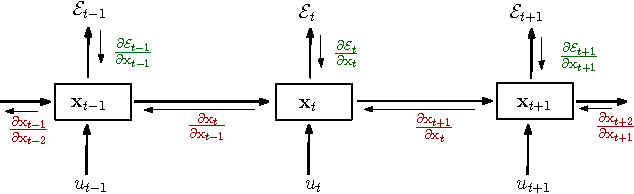
\includegraphics[width=0.8\textwidth]{BPTT}
	\caption[Minh họa thuật toán "Back propagation through time"]{Tại mỗi bước thời gian $t$, đội lỗi không chỉ được lan truyền qua các tầng ở bước thời gian hiện tại mà còn phải lan truyền thông tin độ lỗi qua tất cả thời điểm trước đó. Chính sự lan truyền qua thời gian này gây ra hiện tượng bùng nổ hoặc biến mất gradient.}
	\label{fig_lstmCell}
\end{figure}

Nhắc lại rằng trong RNN, gradient của hàm lỗi tại bước thời gian $t$ theo tham số hồi quy $\theta  \in \{W_{hh}, W_{xh}, b_h \}$ là:
\begin{equation} \label{beginGradientVanish0}
	\nabla_{\theta}L = \frac{\partial L_t}{\partial s_t} \frac{\partial s_t}{\partial h_t} \sum_{r=0}^{t}  \frac{\partial h_t}{\partial h_r}\frac{\partial h_r}{\partial \theta}
\end{equation}
và 
\begin{equation} \label{beginGradientVanish1}
	\frac{\partial h_t}{\partial h_r} = \prod_{i=r}^{t} W_{hh}^T \diag \left( \phi'(h_i) \right)
\end{equation}

Đầu tiên, để cho đơn giản, ta hãy xem $\phi$ là hàm một hàm đồng nhất (identity function) với $\phi(x) = x$ như vậy theo công thức trên, ta có:
\begin{equation} \label{gradientVanish3}
	\frac{\partial h_t}{\partial h_r} = \prod_{i=r}^{t} W_{hh}^T = \left (W_{hh}^T \right)^{t-r}
\end{equation}

Với $W_{hh}$ là một ma trận vuông, nó có thể được phân tích thành dạng:
\begin{equation} \label{gradientVanish4}
	W_{hh} = \Sigma \diag \left(\lambda \right) \Sigma^{-1} 
\end{equation}

Với $\Sigma, \lambda$ lần lượt là ma trận véc-tơ riêng và véc-tơ trị riêng của ma trận $W_{hh}$. Ta biết rằng lũy thừa của $W_{hh}$ cũng chính là lũy thừa của véc-tơ trị riêng của nó $\lambda$. Khi số mũ của phép lũy thừa lớn, những véc-tơ riêng ứng với trị riêng $\lambda_i < 1$ sẽ giảm theo hàm mũ, những véc-tơ riêng ứng với trị riêng $\lambda_i > 1$ sẽ tăng theo hàm mũ. Nói cách khác, \textit{điều kiện đủ} để xảy ra "gradient" biến mất là trị riêng lớn nhất của ma trận kết nối hồi quy $\lambda_{max}$ có giá trị nhỏ hơn 1. Để xảy ra "gradient" bùng nổ, \textit{điều kiện cần} là $\lambda_{max} > 1$.

Trong trường hợp tổng quát với một hàm kích hoạt $\phi$ bất kỳ, với $\phi'$ bị chặn trên bởi $\gamma \in \mathbb{R}$ và do đó $||diag(\phi'(h_k))|| \leq \gamma$. Với $\lambda_{max} < \frac{1}{\gamma}$, hiện tượng "gradient" biến mất sẽ xảy ra. Theo công thức \ref{gradientWRTSt17}:
\begin{equation} \label{gradientVanish5}
	\forall i, \norm{\frac{\partial h_{i+1}}{\partial h_{i}}} \leq \norm{ W^T_{hh} } \norm{ diag(\phi'(h_k)) } < \frac{1}{\gamma} \gamma < 1 
\end{equation}

Đặt $\beta \in \mathbb{R}$ sao cho $\forall i, \norm{\frac{\partial h_{i+1}}{\partial h_{i}}} \leq \beta < 1$, như vậy ta có thể thấy được rằng:
\begin{equation} \label{gradientVanish3}
	\lim_{t - r \to \infty} \frac{\partial h_{t}}{\partial h_r} = \prod_{i=r}^{t} W_{hh}^T \diag \left(\phi'(h_i) \right) \leq \beta^{t - r} = 0
\end{equation}

Bằng cách đảo ngược chứng minh này ta được \textit{điều kiện cần} để xảy ra "gradient" bùng nổ là trị riêng lớn nhất $\lambda_{max}$ lớn hơn $\frac{1}{\gamma}$.

Chứng minh trên cho thấy rằng, khi $t-r$ lớn, tức là khoảng cách giữa từ đang xét và một từ trong quá khứ là lớn thì $\nabla_{\theta_r} L_t$ sẽ hoặc rất bé nếu $\lambda_{max} < \frac{1}{\gamma}$ hoặc có khả năng trở nên rất lớn nếu $\lambda_{max} > \frac{1}{\gamma}$. Trong thực tế, với $\phi$ là hàm \textbf{tanh} ta có $\gamma = 1$ trong khi với $\phi$ là hàm sigmoid, ta có $\gamma = 1/4$. Nếu ta khởi tạo tham số $\theta$ nhỏ hoặc dùng hàm kích hoạt có $\gamma$ nhỏ như hàm \textbf{sigmoid} thì sự biến mất gradient sẽ dễ rất dễ xảy ra; nó khiến cho mô hình chỉ học được những phụ thuộc cục bộ. Ngược lại, nếu $\theta$ được khởi tạo với giá trị lớn, gradient tại các bước thời gian ở xa sẽ bùng nổ và kết quả là mô hình không thể học được \cite{pascanu2011}.

Một kỹ thuật để đối phó với sự bùng nổ gradient được đề là chuẩn hóa gradient về một giá trị nếu nó vượt quá một ngưỡng nào đó. Kỹ thuật này gọi là "gradient clipping" được đề xuất bởi Thomas Mikolov và trình bày lại trong \cite{pascanu2012}. Cụ thể, ta đặt một ngưỡng là chặn trên cho gradient, bất cứ khi nào độ lớn của gradient lớn hơn ngưỡng này ta sẽ chuẩn hóa trở về một giá trị nhỏ hơn. Giải pháp này được áp dụng trong thực tế để ngăn chặn các giá trị \textbf{NaN} (Not a Number) trong gradient và cho phép quá trình huấn luyện tiếp tục. "Gradient clipping" được trình bày trong thuật toán \ref{alg_GDClipping}.

\begin{algorithm}
	\newalgname{Thuật toán}
	\caption{Gradient clipping}
	\label{alg_GDClipping}
	\begin{algorithmic}[1]
		\renewcommand{\algorithmicrequire}{\textbf{Đầu vào:}}
		\renewcommand{\algorithmicensure}{\textbf{Đầu ra:}}
		\algnewcommand\algorithmicoperation{\textbf{Thao tác:}}
		\algnewcommand\Operation{\item[\algorithmicoperation]}
		
		\Require Gradient ứng với tham số $\theta$
		\Ensure Gradient ứng với tham số $\theta$ được chuẩn hóa về một ngưỡng $threshold$
		
		\Operation
		\State $\hat{g} \leftarrow \frac{\partial E}{\partial \theta}$
		\If {$\norm{\hat{g}} \geq threshold$}
			\State $\hat{g} \leftarrow \frac{threshold}{\norm{\hat{g}}} \hat{g}$
		\EndIf
	\end{algorithmic}
\end{algorithm}

\section{Long short-term memory (LSTM)}

\begin{figure}
	\centering
	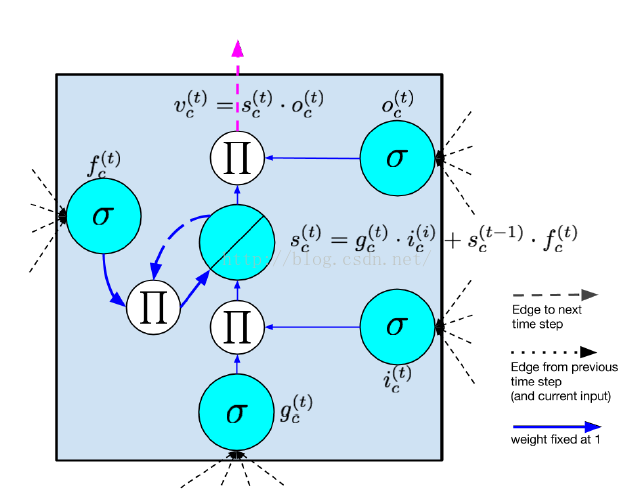
\includegraphics[width=0.6\textwidth]{lstmCell}
	\caption[Một "LSTM cell"]{Mô hình RNN đơn giản với kết nối vòng, \textbf{$h$} được xem như bộ nhớ được luân chuyển trong RNN. Chú ý rằng đường nét đứt ở đầu ra thể hiện rằng tại một thời điểm $t$, RNN có thể có hoặc không có một đầu ra.}
	\label{fig_lstmCell}
\end{figure}

Hochreiter và Schmidhuber \cite{hochreiter1997} đã giới thiệu mô hình \textit{Long short-term memory} (LSTM) chủ yếu ở để khắc phục vấn đề biến mất gradient trong RNN. Nhớ lại rằng trong RNN, chính việc mô hình hóa phụ thuộc thời gian dựa vào ma trận trọng số $W_{hh}$ đã gây ra hiện tượng gradient biến mất. Giả sử gọi $S_t$ là trạng thái liên kết hồi quy (trong RNN, nó chính là trạng thái ẩn). Ý tưởng của LSTM là thay vì tính toán $S_t$ từ $S_{t-1}$ với một phép nhân ma trận theo sau là hàm kích hoạt phi tuyến, LSTM trực tiếp tính toán một $\Delta S_t$ sau đó nó được cộng với $S_{t-1}$ để tạo ra $S_t$. Thoạt nhìn, sự khác biệt này có thể không đáng kể khi mà chúng ta đều đạt được $S_t$ trong cả hai cách. Tuy nhiên, với cách làm này, các "gradient" của LSTM tính toán $\Delta S_t$ sẽ không bị biến mất.

Thuật ngữ "Long short-term memory" xuất phát từ nhận định sau. Mạng RNN đơn giản có "long term memory" (bộ nhớ dài hạn) dưới dạng các ma trận trọng số. Những ma trận trọng số này thay đổi một cách chậm rãi trong quá trình học nhằm mã hóa kiến thức về dữ liệu. RNN cũng có "short-term memory" (bộ nhớ ngắn hạn) dưới dạng các kích hoạt tạm thời, được truyền từ mỗi bước thời gian sang các bước thời gian sau đó. "Long short-term memory" tạm dịch là "bộ nhớ ngắn hạn dài" cho phép mở rộng bộ nhớ ngắn hạn bằng cách thêm vào một loại lưu trữ trung gian gọi là trạng thái lưu giữ (cell state). Trạng thái lưu giữ này có khả năng lưu giữ các thông tin cần thiết một cách lâu dài dưới dạng một bộ nhớ ngắn hạn. Để làm được điều này, LSTM sử dụng một cơ chế gọi là "cổng", các "cổng" giúp được huấn luyện để chọn lọc thông tin nào là cần thiết để tác động lên trạng thái lưu trữ. Với cách làm này, trạng thái lưu trữ sẽ lưu được nhiều thông tin hơn, vì chỉ những thông tin quan trọng mới tồn tại trong nó.

Về cấu tạo, một LSTM tương tự như một RNN một lớp ẩn, nhưng mỗi "RNN cell" (ký hiệu "A" trong hình \ref{fig_rnn_unrolled}) được thay thế bằng một "memory cell" (hình \ref{fig_lstmCell}). Giống như "RNN cell", "memory cell" nhận một đầu vào bên ngoài và phát sinh một đầu ra cũng như là truyền đi một trạng thái ẩn sang "memory cell" ở bước thời gian kế tiếp. Tuy nhiên, trong "memory cell" còn có thêm một trạng thái lưu giữ cũng được truyền đi như một trạng thái ẩn. Cấu tạo chi tiết của LSTM sẽ được trình bày trong phần dưới đây, cấu tạo này dựa trên phiên bản LSTM của \cite{gers2000}.

\begin{itemize}
	\item[•] \textit{Nút đầu vào (input node)}: Đơn vị này được ký hiệu là $g$, là một mạng nơ-ron một tầng ẩn. Nút đầu vào có nhiệm vụ mô hình hóa đầu vào tại mỗi bước thời gian. Nó nhận tham số là đầu vào tại bước thời gian hiện tại $x_t$ và trạng thái ẩn tại thời điểm trước đó $h_{t-1}$. Cụ thể, tại mỗi bước thời gian nút đầu vào có công thức:
	\begin{equation} \label{inputNodeLSTM}
		g_t = \phi \left(W_{gx}x_t + W_{gh}h_{t-1} + b_g \right)
	\end{equation}
	\item[•] \textit{Cổng vào (input gate)}: "Cổng" như đã nói, là một cơ chế đặc biệt của LSTM. Cổng vào cũng được cấu tạo giống như nút đầu vào, nó nhận tham số là $x_t$ và $h_{t-1}$. Sau đó được đưa qua hàm kích hoạt $\sigmoid$ để tạo ra giá trị trong khoảng $(0,1)$. Sở dĩ đơn vị này được gọi là "cổng vào" vì giá trị của nó sẽ được sử dụng để nhân với giá trị của nút đầu vào. Giá trị của nó thể hiện lượng thông tin mà nút đầu vào được phép truyền đi. Nếu cổng vào bằng 0, nút đầu vào sẽ truyền đi với giá trị 0. Nếu cổng vào bằng 1, nút đầu vào sẽ truyền đi với giá trị ban đầu. Cụ thể hơn, ta có công thức của cổng vào, được ký hiệu là $i$, tại bước thời gian $t$:
	\begin{equation} \label{inputGateLSTM}
		i_t = \sigma \left(W_{ix}x_t + W_{ih}h_{t-1} + b_i \right)
	\end{equation}
	\item[•] \textit{Trạng thái lưu giữ (cell state)}: Trái tim của LSTM chính là trạng thái lưu trữ, là một mạng nơ-ron với hàm kích hoạt tuyến tính. Khá giống với trạng thái ẩn trong RNN, trạng thái lưu trữ $s_t$ cũng có một kết nối hồi quy với trạng thái lưu trữ trước đó $s_{t-1}$. Tuy nhiên, trọng số kết nối hồi quy luôn có giá trị cố định là 1. Bởi vì kết nối hồi quy này qua nhiều bước đều có trọng số không đổi nên khi tính toán, "gradient" của độ lỗi không bị bùng nổ hay biến mất. Tại mỗi bước thời gian, trạng thái lưu trữ được tính như sau:
	\begin{equation} \label{cellStateLSTM}
		s_t = s_{t-1} + g_t \odot i_t
	\end{equation}
	\item[•] \textit{Cổng quên (forget gate)}: Cổng quên là một đề xuất của \cite{gers2000} so với bài báo LSTM gốc. Thay vì kiểm soát lượng thông tin để đưa vào trạng thái lưu giữ như cổng vào, cổng quên cung cấp khả năng tẩy đi một lượng thông tin trong trạng thái lưu giữ. Cụ thể, cổng quên với giá trị thuộc khoảng $(0,1)$ sẽ được nhân với $s_{t-1}$ trong công thức \ref{cellStateLSTM}. Tại mỗi bước thời gian, giá trị của cổng quên $f_t$ được tính như sau:
	\begin{equation} \label{forgetGateLSTM}
		f_t = \sigma \left(W_{fx}x_t + W_{fh}h_{t-1} + b_f \right)
	\end{equation}
	Công thức của trạng thái lưu trữ được sửa lại khi có cổng quên:
	\begin{equation} \label{cellStateWithForgetGateLSTM}
		s_t = s_{t-1} \odot f_t + g_t \odot i_t
	\end{equation}
	\item[•] \textit{Cổng ra (output gate)}: Giá trị đầu ra $v_t$ của "memory cell" tại mỗi bước thời gian chính là tích giá trị của trạng thái lưu trữ $s_t$ với giá trị của cổng ra $o_t$. Trong một số phiên bản của LSTM, hàm kích hoạt $\phi$ có thể là hàm \textbf{tanh} hoặc \textbf{sigmoid} hoặc không sử dụng hàm kích hoạt nào. Tại mỗi bước thời gian, giá trị của cổng ra $o_t$ được tính như sau:
	\begin{equation} \label{outputGateLSTM}
		o_t = \sigma \left(W_{ox}x_t + W_{oh}h_{t-1} + b_o \right)
	\end{equation}
	Đầu ra của "memory cell" cũng chính là trạng thái ẩn $h_t$ có giá trị:
	\begin{equation} \label{outputNodeLSTM}
		h_t = \phi(s_t) \odot o_t 
	\end{equation}
\end{itemize}

\section{Mô hình ngôn ngữ}

\subsection{Mô hình ngôn ngữ \textit{n}-gram}

Như chúng tôi đã đề cập trong chương 1, \textit{mô hình ngôn ngữ} (language model) là một bộ phận quan trọng trong cả dịch máy thống kê và dịch máy nơ-ron. Nó giúp ta dự đoán được từ tiếp theo trong một chuỗi từ cho trước. Cụ thể hơn, mô hình ngôn ngữ là một phân phối xác suất trên một chuỗi các từ. Cho trước một chuỗi $w_1,w_2,...,w_n$ (ký hiệu $w_{1:n}$), mô hình ngôn ngữ gán cho nó một xác suất $p(w_{1:n})$ đại diện cho độ "trơn tru" của chuỗi đó. Theo công thức xác suất có điều kiện, ta có:
\begin{equation} \label{traditionalLM}
\begin{split}
	p(w_{1:n}) &= p(w_1)p(w_2|w_1)p(w_3|w_{1:2})...p(w_n|w_{1:n-1}) \\
				&= \prod_{t=1}^{n} p(w_t|w_{1:t-1})
\end{split}
\end{equation}
 
Trong công thức trên, mỗi thành phần $p(w_i|w_{1:i})$ là xác suất có điều kiện của từ $w_i$ biết những từ trước đó $w_{1:i}$, những từ này còn được gọi là ngữ cảnh đối với từ đang xét. Ta thấy rằng để tính được xác suất $p(w_i|w_{1:i})$ ta phải xét đến tất cả những từ đứng trước nó. Điều này làm cho chi phí tính toán trở nên rất lớn. Để giảm chi phí tính toán, người ta sử dụng giả định \textit{markov} (markov-assumption); giả định này nói rằng các từ tiếp theo chỉ liên quan đến từ hiện tại và độc lập với các từ trước đó. Chính xác hơn, một giả định markov bậc $k$ nói rằng từ tiếp theo trong một chuỗi chỉ phụ thuộc vào $k$ từ cuối cùng trong chuỗi.
\begin{equation} \label{markovAssumption}
	p(w_{i+1}|w_{1:i}) \approx p(w_{i+1}|w_{i-k:i})
\end{equation}

Công thức \ref{traditionalLM} theo giả định markov trở thành:
\begin{equation} \label{traditionalLM}
	p(w_{1:n}) = \prod_{t=1}^{n} \approx p(w_{i-k}|w_{i-k:i-1})
\end{equation}

Mặc dù giả định markov bậc $k$ rõ ràng là sai với $k$ bất kỳ (một câu có thể có phụ thuộc dài hạn với chiều dài bất kỳ như câu bắt đầu bằng từ \textit{what} và kết thúc bằng dấu \textit{?}), tuy nhiên nó vẫn tạo ra những mô hình ngôn ngữ mạnh mẽ với với các giá trị tương đối nhỏ của $k$ ($k=3$ hoặc $k=5$), và là phương pháp chủ yếu cho bài toán mô hình hóa ngôn ngữ trong hàng thập kỷ.

Cách tiếp cận truyền thống cho bài toán mô hình hóa ngôn ngữ là sử dụng mô hình ngôn ngữ \textit{n}-gram. Sở dĩ nó có tên như vậy là vì nó sử dụng giả định markov bậc \textit{n} - 1 để ước lượng xác suất $p \left(w_{i+1}=m|w_{1:i} \right) \approx p \left(w_{i+1}=m|w_{i-(n-1):i} \right)$. Theo mô hình ngôn ngữ \textit{n}-gram, xác suất để từ $m$ theo sau chuỗi các từ $w_{1:i}$ là:

\begin{equation} \label{ngramLM}
	p \left(w_{i+1}=m|w_{i-(n-1):i} \right) = \frac{\# \left(w_{i-(n-1):i+1} \right)}{\# \left(w_{i-(n-1):i} \right)}
\end{equation}
trong đó $\#(w_{i:j})$ là số lần xuất hiện của chuỗi $w_{i:j}$ trong tập ngữ liệu. Các mô hình \textit{n}-gram thông thường sử dụng $n = 2$ và $n = 1$ được gọi lần lượt là mô hình \textit{trigram} và mô hình \textit{bigram}. Trong trường hợp mô hình không sử dụng ngữ cảnh để ước lược lượng xác
suất của một từ ($n = 0$), thì mô hình này được gọi là mô hình \textit{unigram}.

Bên cạnh sự hiệu quả, phương pháp này có một khuyết điểm lớn: nếu chuỗi $w_{i-(n-1):i+1}$ chưa từng xuất hiện trong tập ngữ liệu, tức $\# \left(w_{i-(n-1):i+1} \right) = 0$ thì xác suất ước lượng sẽ có giá trị bằng 0. Điều này dẫn đến xác suất của toàn bộ chuỗi cũng bằng 0 do phép nhân trong công thức tính của nó (công thức \ref{traditionalLM}). Việc xác suất bằng 0 xảy ra khá thường xuyên do sự giới hạn của tập ngữ liệu.

Một cách để tránh việc xảy ra các sự kiện xác suất bằng không là sử dụng những kỹ thuật \textit{làm mịn} (smoothing techniques). Làm mịn bảo đảo tất cả mọi chuỗi đều có một xác suất xuất hiện (mặc dù nhỏ). Kỹ thuật làm mịn đơn giản nhất là làm mịn thêm $\alpha$ (add-$\alpha$ smoothing) \cite{goodman2001}; nó bảo đảm bất kỳ chuỗi nào cũng xuất hiện ít nhất $\alpha$ lần. Với làm mịn thêm $\alpha$ ta được:
\begin{equation} \label{ngramLMWithSmoothing}
	p_{add-\alpha} \left(w_{i+1}=m|w_{i-k:i} \right) = \frac{\# \left(w_{i-(n-1):i+1} \right) + \alpha}{\# \left(w_{i-(n-1):i} \right) + \alpha \left|V \right| }
\end{equation}
trong đó $\left|V \right|$ là số lượng từ vựng trong tập ngữ liệu.

Một kỹ thuật khác bên cạnh làm mịn là kỹ thuật \textit{truy hồi} (back-off): nếu chuỗi \textit{n}-gram chưa từng xuất hiện trong tập ngữ liệu thì chúng ta sẽ tính xác suất của chuỗi dựa trên (\textit{n - }1)-gram. Chúng ta tiếp tục truy hồi cho đến khi chúng ta gặp một chuỗi mà tần xuất của nó khác không. Ví dụ với trường hợp \textit{trigram}:
\begin{equation} \label{ngramLMKatzBackoff1}
\begin{split}
	p_{bo} \left(w_{i+1}=m|w_{i-1}, w_{i-2} \right) = \lambda_1 p \left(w_{i+1}=m|w_{i-1}, w_{i-2} \right) \\ 
	+ \lambda_2 p \left(w_{i+1}=m|w_{i-2} \right) \\ 
	+ \lambda_3 p \left(w_{i+1}=m \right)
\end{split}
\end{equation}
trong đó các $\lambda$ có tổng là $1$:
\begin{equation} \label{ngramLMKatzBackoff2}
\sum_{i} \lambda_i = 1
\end{equation}









